\documentclass[conference,compsoc]{IEEEtran}

\ifCLASSOPTIONcompsoc

  \usepackage[nocompress]{cite}
\else
  \usepackage{cite}
\fi


\usepackage{graphicx}
\usepackage{fixltx2e}
\usepackage{float}
\graphicspath{ {E:/faculta/Master/DissertationProject/images/} }

\ifCLASSINFOpdf
  
\else
 
\fi

\hyphenation{op-tical net-works semi-conduc-tor}


\begin{document}

\title{An empirical study on the interplay between structural and logical\\ dependencies of software systems classes 
}


\author{\IEEEauthorblockN{Stana Adelina Diana}
\IEEEauthorblockA{Computer Science and Engineering Department\\
"Politehnica" University of Timisoara }
\and
\IEEEauthorblockN{Ioana Sora}
\IEEEauthorblockA{Computer Science and Engineering Department\\
"Politehnica" University of Timisoara }}

\maketitle

\begin{abstract}
Software systems are continuously in change. This changing process is never finished as long as the software system is used, changes can be triggered by new features , defects, new technologies, system refactoring for maintainability.\\ Software maintenance can be made during the development process by maintaining the already implemented features while developing new ones or at the end of the development process when the system is no longer open to new features requested by the client and the maintenance is only made for the existing ones. \\From an architectural point of view, a system is stable when a change in one component of the system does not affect the other components .This rule applies recursively also inside the components. The ideal situation will be to be able to make a change in one part without changing parts that are in a dependency relation with that part. Those dependencies affect the maintainability of the system and increase the realization effort of any problem that appears during the maintenance time.\\Studying only the structural dependencies of the system is not enough to get a clear overview of the system dependencies. For more precise results a study that combines structural dependencies and logical dependencies is needed. We have analysed 20 open-source software systems of different sizes to investigate the links between structural dependencies and logical dependencies.
\end{abstract}

\IEEEpeerreviewmaketitle

\section{Introduction}
During the development process of a software system new classes and new methods to the existing classes are added in order to fulfill new functionalities. All of the adding actions from above have a direct impact on the system structural dependencies. Structural dependencies are dependencies that result following the source code analysis of the system. The source code is any static, textual, human readable, fully executable description of a computer program that can be compiled automatically into an executable form\cite{ct1} .\\ On the other hand logical dependencies also can be added during the development process. Logical dependencies refer to those depencencies between entities that are not always visible through source code analysis (Figure \ref{fig:fig1}).
\begin{figure}[H]
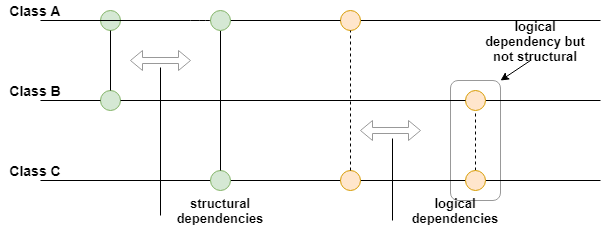
\includegraphics[scale=0.45]{fig1.png}
\caption{Relationships between structural and logical dependencies }
\label{fig:fig1}
\centering
\end{figure}
Logical dependencies can be easily extracted from the versioning system (e.g. Subversion , Git) commits. When building the logical dependencies we have not taken into consideration classes that co-change only by comment changes. For a change to be taken into consideration in creation a new logical link it had to involve code change.  In this paper we intend to understand better the intersection between structural dependencies and logical dependencies and it's impact over the system (Figure \ref{fig:fig2}). 
\begin{figure}[H]
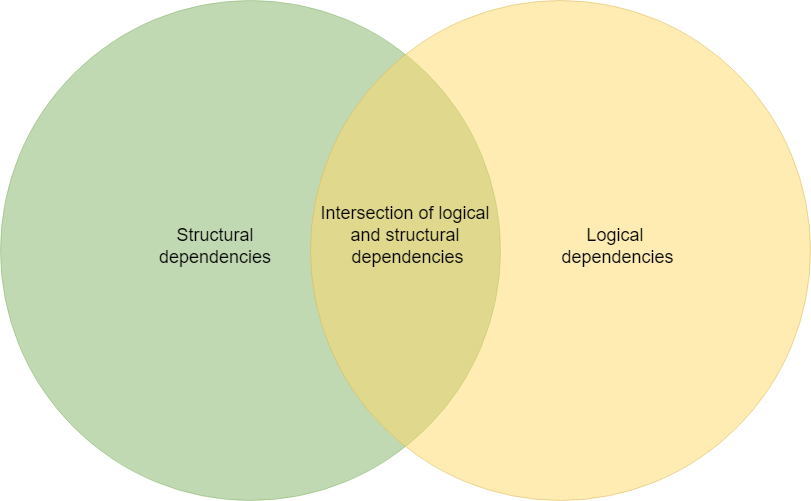
\includegraphics[scale=0.35]{fig2.png}
\caption{Venn Diagram showing the intersection between structural and logical dependencies }
\label{fig:fig2}
\end{figure}
\begin{figure*}[h]
\centering
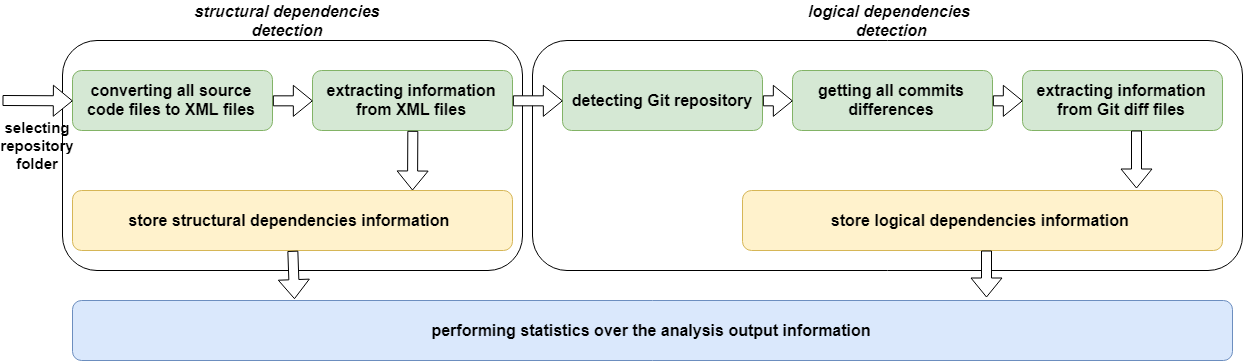
\includegraphics[width=\textwidth]{fig3.png}
\caption{Processing phases}
\label{fig:fig3}
\end{figure*}
\section{Tool for measuring software dependencies}
 A dependency is created by two elements that are in a relationship and indicates that an element of the relationship, in some manner, depends on the other element of the relationship. In this case, if one of these elements change, there could be an impact to the other \cite{ct2}. Dependencies are discovered by analysis of source code or from an intermediate representation such as abstract syntax trees \cite{ct3} .\\
In order to build structural and logical dependencies we have developed a tool that takes as input the source code repository and builds the required software dependencies . The workflow can be delimited by three major steps as it follows (Figure \ref{fig:fig3}):\\ \\
\textit{\textbf{Step 1:} Extracting structural dependencies.}\\
\textit{\textbf{Step 2:} Extracting logical dependencies.}\\
\textit{\textbf{Step 3:} Processing the information extracted.}\\


In the next subsections we introduce the notion of structural dependencies and how it can be identified trough the source code of the system and the notion of logical dependencies and how it can be idenfied trough the commits from the versioning system.

\subsection{ Structural dependencies}
\subsubsection{ Definition }
Structural dependencies (a.k.a syntactic dependencies or structural coupling) are the result of source code analysis. Each source code file can contain one or more classes. \\There are several types of relationships between source code entities, a method can call another class method, a class extends another class, all those create dependencies between classes \cite{ct4}.\\ Even though in some of the cases if class A depends on class B , changes in class B can produce changes in class A, but not the other way around \cite{ct5} . There are other cases in which if class A depends on class B,  changes in class B can produce changes in class A and viceversa if we are speaking in the context of a new feature implementation that implies changing return types and adding new methods.So we will consider structural dependencies as bidirectional relationship, "class A depends on class B" and "class B depends on class A". \\The choice of building bidirectional relationships is motivated by the fact that we cannot establish for the moment the direction of the logical dependencies of the system. So in order to have a omogeninty between the logical and structural dependencies analysis results, we will take both of the relationships types as bidirectional. 
\subsubsection{ Extracting structural dependencies }
As mentioned above the first step of analysis is to extract structural dependencies. In this step the entire source code folder is scanned and only source code files are extracted in order to convert them into XML files (a.k.a  Extensible Markup Language files), for each source code file an XML file is made. The process of converting source code files to XML file is made through calls to an external tool called srcML. The motivation behind converting into XML representation of source code is that explicitly embeds the syntactic structure present in source code text with XML tags \cite{ct9}. All the information about classes, methods, calls to other classes is stored internally and afterwards stored together with the information extracted from versioning system revisions into an XML file. The tool gives the possibility to upload the XML file mentioned previously in order to skip the source code and revisions processing and directly switch to the statistics reporting phase.

\subsection{ Logical dependencies}
\subsubsection{ Definition }
Co-evolution is a terminology used in biology to indicate change in the genetic composition of one species in response to a genetic change in another \cite{ct5}. \\In software engineering, co-evolution represents the phenomenon through one component changes in response to a change in another component. Those changes can be found in the software history \cite{ct6}. \\  Logical dependencies (a.k.a logical coupling) are the result of software history analysis and can reveal relationships that are not present in the source code code (structural depencencies). If class A depends only on class B  and class D has no structural connection with class A and B but each time class D changes also class A changes then class A and D have a logical relationship. Not all the relationships that result from software history analysis are not included in the structural analysis relationships, most likely if class A depends on class B then during the evolution of the system class A and class B will change together.
\subsubsection{ Extracting logical dependencies }
The second step of the analysis is to extract logical dependencies from the versioning system.\\The versioning system contains the long-term change history of every file. Changes can be made by many individuals over the years. Changes include the creation and deletion of files as well as edits to their contents. Each change (this can include changes in multiple files) made by an individual at certain point of time is contained into a revision  \cite{ct7}. All the revisions are stored in the versioning system cronologicaly and each revision has a parent revision. The parent revision is the revision from which development began, the only exeption to this rule is the first revision which has no parent revision. We will take into consideration only revisions that have a parent revision since the first revision can include source code files that are already in development (migration from one versioning system to another) and this can introduce reduntant logical links .\\ We also will take into consideration only revisions that contain changes in at least one file with .java extension since our main focus is finding classes that change together that can only be contained in .java files \cite{ct8} .\\ The tool looks through the repository and gets all the existing revisions, for each revision a differences file will be made . The differences file will contain all the changes from all the files merged . Before making the differences file, the revision shall fulfill all the conditions mentioned above. In addition each file will be saved with the number of .java files changed in his name. In this way it will be more easy to filter the revisions differences files by the number of files changed.\\ Finally after all the differences files are stored , all the files are parsed and logical dependencies are build. The logical dependencies are splitted into three categories : dependencies found in revisions with less than 5 files changed, dependencies found in revisions with more than 5 files changed but less than 20 and dependencies found in revisions with more than 20 files changed. Also dependencies found with only comments change where not taken into consideration (class A and class B change together but the only change found is in comments).

\section{Experimental results}

\section{Conclusion}


\begin{thebibliography}{1}

\bibitem{ct1}
David Binkley, \emph{Source Code Analysis: A Road Map}, Future of Software Engineering, 2007. FOSE '07.
\bibitem{ct2}
G. Booch, \emph{Object-Oriented Analysis and Design with Applications}, Third Edition: Addison-Wesley, 2007.
\bibitem{ct3}
Marcelo Cataldo, Audris Mockus, Jeffrey A. Roberts, and James D. Herbsleb, \emph{Software Dependencies, Work Dependencies, and Their Impact on Failures},  IEEE Transactions on Software Engineering ( Volume: 35, Issue: 6, Nov.-Dec. 2009 ), pp. 864-878.
\bibitem{ct4}
Beck F., Diehl S.,\emph{ On the congruence of modularity and code coupling}, In ESEC/FSE'11: European Software Engineering Conference and Symposium on Foundations of Software Engineering (2011), pp. 354-364.
\bibitem{ct5}
Liguo Yu,\emph{Understanding component co-evolution with a study on Linux}, Empirical Software Engineering, April 2007, Volume 12, Issue 2, pp. 123-141.
\bibitem{ct6}
Igor Wiese, Rodrigo Kuroda, Reginaldo Re, Gustavo Oliva, Marco Gerosa, \emph{An Empirical Study of the Relation Between Strong Change Coupling and Defects Using History and Social Metrics in the Apache Aries Project}, IFIP International Conference on Open Source Systems, OSS 2015: Open Source Systems: Adoption and Impact, pp. 3-12.
\bibitem{ct7}
 Ben Collins-Sussman, Brian W. Fitzpatrick, and C. Michael Pilato, \emph{Version Control with Subversion}, http://svnbook.red-bean.com/en/1.7/svn.basic.version-control-basics.html, 2008.
\bibitem{ct8}
N. Ajienka and A. Capiluppi,  \emph{Understanding the interplay between the logical and structural coupling of software classes}, J. Systems Software, vol. 134, pp. 120-137, 2017.
\bibitem{ct9}
 Huzefa Kagdi, Malcom Gethers, Denys Poshyvanyk, Michael L. Collard,\emph{Blending Conceptual and Evolutionary Couplings to Support Change Impact Analysis in Source Code}, 17th Working Conference on IEEE, 2010, pp. 119-128.

\end{thebibliography}

\end{document}


